\chapter{Cálculos}\label{cap:calculus}

\section{Cálculo para aleta Infinita}\label{sec:infity}

Realizado análize para aleta Infinita, obtida através da relação:\\
\begin{equation}
    {m}{L}\geq{2,65}
\end{equation}
\begin{equation}
    {L}\geq{\frac{2,65}{m}}
\end{equation}
\begin{equation}
    {L}\geq{\frac{2,65}{12,311 }}
\end{equation}
\begin{equation}
    {L}\geq{0,21522496\,\SI{}{\meter}}
\end{equation}
\par Para que hipótese da aleta infinita fosse válida, a aleta deveria ter um
comprimento maior ou igual a 21,522496 cm.
Neste caso a geometria 3 apresenta comprimento menor, embasando a
escolha da utilização do cálculo de contorno A.

\section{Determinar a temperatura da superfície da base da aleta (Tb)}\label{sec:prob1}

\begin{equation}
    {qx}={\frac{T\infty-Ts1}{1/{h1}}}={\frac{Ts1-Ts2}{L/{{k}{A}}}}={\frac{Ts2-T\infty2}{1/{h2}{A}}}
\end{equation}

\begin{figure}[h]
    \centering
    \caption{Representação das resistências térmicas.}
    \label{fig:res}
    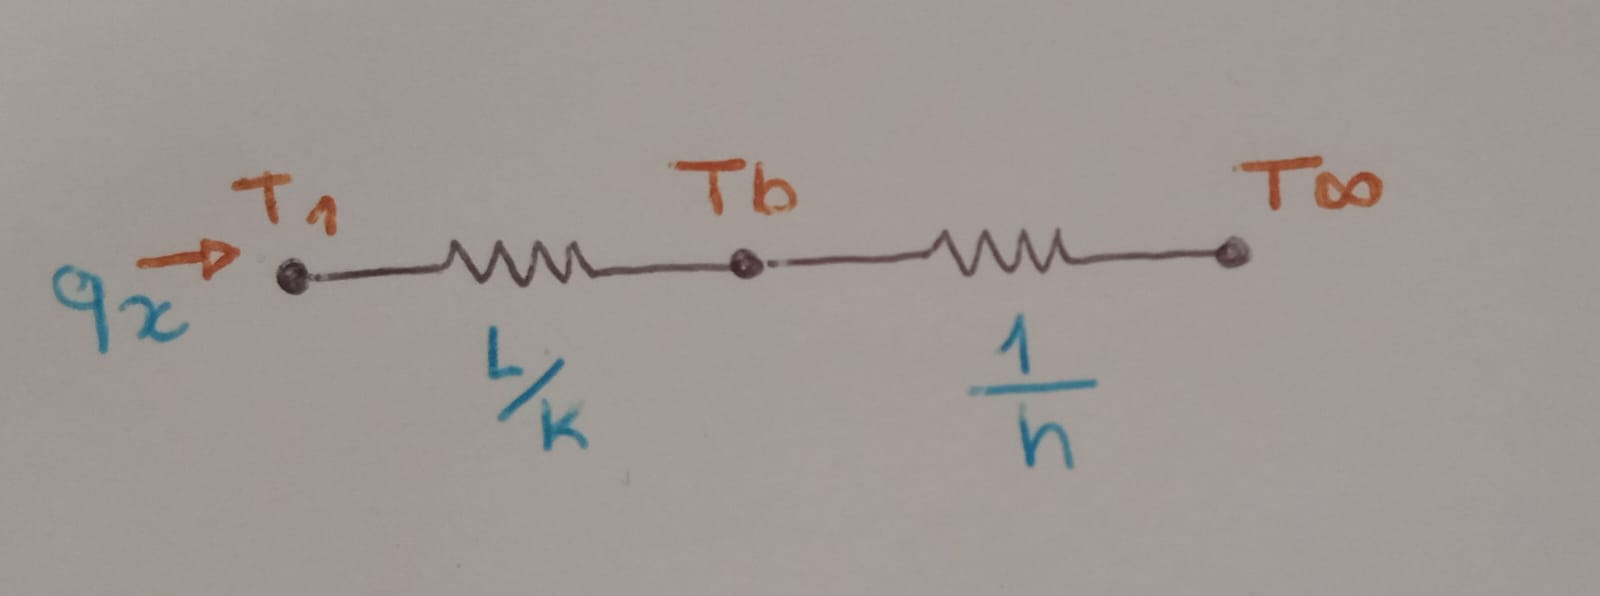
\includegraphics[width=14cm]{figuras/resistenciasTermicas.jpeg}
    \fonteproprioautor
\end{figure}

Isolando o Tb chegamos ao resultado de:
\begin{equation}
    {Tb}={\frac{T1 -T\infty}{{R1}+{R2}}}-{T1} = \SI{109,989}{\degreeCelsius}
\end{equation}

\clearpage

\section{Determinar a taxa de transferência de calor de cada tipo de aleta (qa)}\label{sec:calcTable}

\begin{figure}[h]
    \centering
    \caption{Tabela com condições de cálculos para superfícies estendidas.}
    \label{fig:tabelaCasosCalc}
    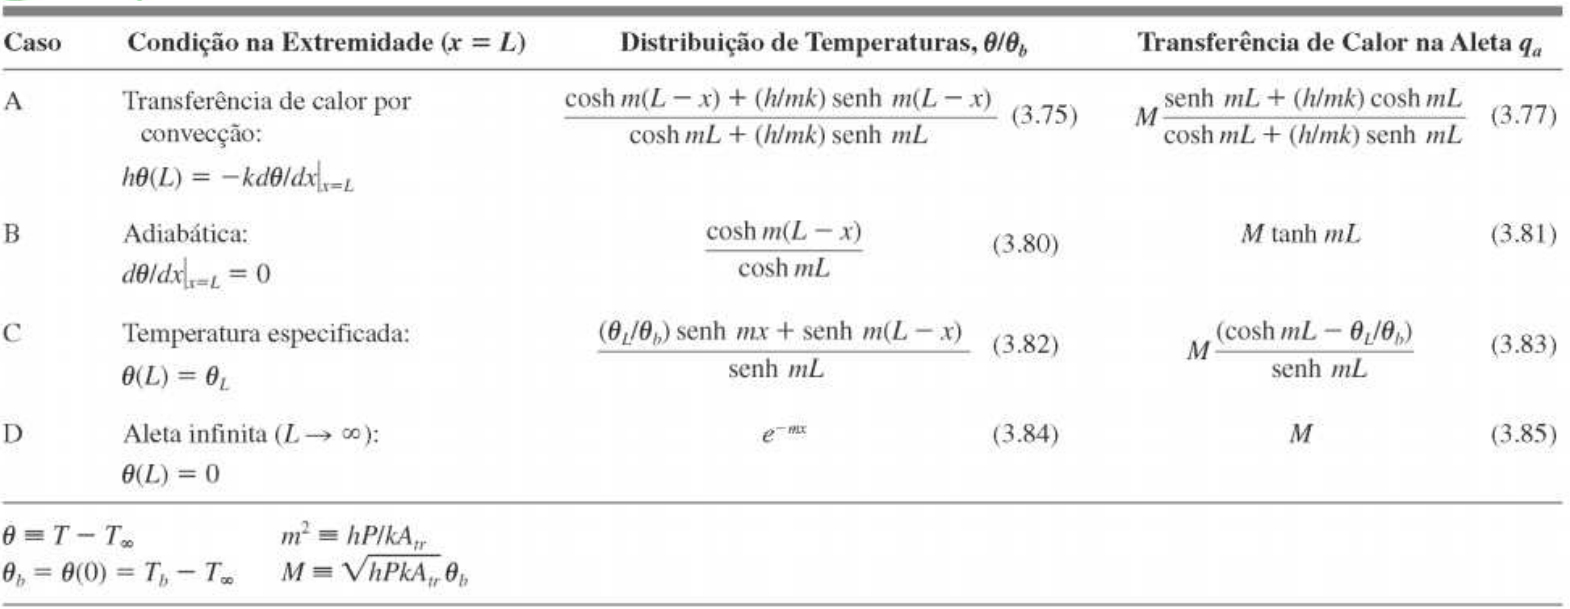
\includegraphics[width=15cm]{figuras/tabelaCasosCalc.jpg}
    \fonte{\cite{antonietti}}
\end{figure}

Foi escolhida a equações do caso \(A\), pelo fato das equações
\(D\) aleta inifita resultar em um valor muito acima do comprimeto da
geometria,
\(B\) por não conter superfícies adiabáticas
e \(C\) por não conter uma temperatura especificada na parcela estendida.
\par No caso da equação \(A\), necessita-se dos seguintes valores
para prosseguimento com os cálculos:
\begin{itemize}[leftmargin=2cm]
    \item Perímetro da aleta: \(
          {P}={2w+2t} = \SI{10,8}{\milli\meter}
          \)
    \item Diferença de temperatura: \(
          {\theta}b={{Tb}-{T\infty}} = \SI{79,989}{\degreeCelsius}
          \)
    \item Área da seção transversal da aleta: \(
          {Atr}={{w}{t}} = \SI{12,311}{\per\meter}
          \)
    \item Valor \(M\): \(
          {M}={\sqrt[]{{h}{P}{k}{Atr}}} = \SI{1,403}{\watt}
          \)
    \item Taxa de transferência
          de calor da aleta: \\\(
          {qa}={M}{
          \frac
          {\sinh{(mL1)}+{\frac{(h)}{(mk)}}{\cosh{(mL1)}}}
          {\cosh{(mL1)}+{\frac{(h)}{(mk)}}{\sinh{(mL1)}}}
          }={0,3223\,\SI{}{\watt}}
          \)
\end{itemize}

\section{Determinar a temperatura na
  ponta da aleta}\label{sec:C}
\begin{equation}
    {\frac{\theta}{{\theta}b}}=
    {\frac
    {T(x)-{T\infty}}
    {Tb-{T\infty}}
    }=
    {
    \frac
    {\cosh{(m(L-x))}+{\frac{(h)}{(mk)}}{\sinh{(m(L-x))}}}
    {\cosh{(mL)}+{\frac{(h)}{(mk)}}{\sinh{(m(L-x))}}}
    }
\end{equation}
Isolando o \(tx\) obtém-se:
\begin{equation}
    {Ta(x)}=
    {
    \frac
    {\cosh{(m(L-x))}+{\frac{(h)}{(mk)}}{\sinh{(m(L-x))}}}
    {\cosh{(mL)}+{\frac{(h)}{(mk)}}{\sinh{(m(L-x))}}}
    }+
    {\theta}+
    {T\infty}=
    \SI{107,839}{\degreeCelsius}
\end{equation}

\clearpage

\section{ Determinar a efetividade (\(\epsilon\)) da
  superfície estendida}\label{sec:d}

\begin{equation}
    {{\epsilon}a}=
        {
            \frac
            {{qa1}}
            {{h}{Atrb}{\theta}b}
        }=
        {\SI{33,613}{}}
\end{equation}
\par Não houve a necessidade de realizar melhorias, pois \({\epsilon}a>{2}\).

\section{
  Determinar a eficiência da aleta (\(\eta\)a)
 }\label{sec:e}

\begin{itemize}[leftmargin=2cm]
    \item Áreas das aletas: \(
          {Aa}={{L1}{P}+{Atr}} = 0,0002058131\,\SI{}{\square\meter}
          \)
    \item Eficiência da aleta: \(
          {\eta}a=
          {\frac{qa}{{h}{Aa1}{\theta}b}}{100\%}=
          {\SI{98,20}{\percent}}
          \)
\end{itemize}

\section{
  Determinar a eficiência global
  do conjunto aletado (\(\eta\)o)
 }\label{sec:f}

\par O conjunto aletado global compreende toda a geometria desde a base até todas as superfícies estendidas e 
para determinarmos a eficiência de todo esse conjunto
apenas necessita-se somar a energia transmitida da base
como a energia dissipada por todas as aletas.
A eficiência provem da razão entre da energia  dissipada e a energia dissipada por convecção:

\begin{itemize}[leftmargin=2cm]
    \item Área total (aletas + espaço sem aletas): \(
          {At}={{Aa}{N}+{Ab}} = {0,0112849}\,\SI{}{\square\meter}
          \)
    \item Taxa total da transferência de calor: \(
          {qt}=
          {{N}{{\eta}a}{h}{Aa}{{\theta}b}}+{{h}{Ab}{{\theta}b}}=
              {17,769\,\SI{}\watt}
          \)
    \item Eficiência global do conjunto aletado: \(
          {\eta}o=
          {\frac{qt}{{h}{At}{\theta}b}}{100\%}=
          {\SI{98,43}{\percent}}
          \)
\end{itemize}

\section{
  Resultados
 }\label{sec:results}

O resultados foram satisfatórios pois a aleta apresentou valores de:
\begin{itemize}[leftmargin=2cm]
    \item Efetividade \boldmath\(> 2\), não havendo a necessidade realizar melhorias;
    \item Eficiência global de \boldmath\(98,43\,\%\).
\end{itemize}